% arara: pdflatex
% arara: pdflatex
\RequirePackage{silence}
\WarningsOff[latex]
\documentclass[a4paper,11pt]{report}
\usepackage[a4paper, twoside, left=4.2cm, right=2.4cm, top=3.0cm, bottom=3.3cm]{geometry}


\usepackage{palatino}
\usepackage{multicol}
\usepackage{comment}
%\usepackage[activate={true,nocompatibility},final,tracking=true,kerning=true,spacing=true,factor=1100,stretch=10,shrink=10]{microtype}


% def examples:
\def \shout [#1]#2#3{You are calling def shout with first argument #1,
    second argument #2,
    and third argument #3.}
\def\<{\left\langle}
\def\>{\right\rangle}
\def\fl#1{\left\lfloor #1 \right\rfloor}
\def\cA{{\mathcal A}}

% increases skips by a bit
\usepackage{setspace}
\setstretch{1.2}

%fncychap
\usepackage[Bjornstrup]{fncychap}

\begin{comment}
\usepackage{fancyhdr}
\pagestyle{fancy}
\lhead{}
\chead{\rightmark}
\rhead{}
\lfoot{\leftmark}
\cfoot{}
\rfoot{\thepage}
\end{comment}

\usepackage{tikz}
\usepackage[explicit]{titlesec}

\definecolor{lavender}{rgb}{0.9, 0.9, 0.98}
\definecolor{mediumpurple}{RGB}{147,112,219}
\definecolor{orangered}{RGB}{255,165,0}

\begin{comment}
\titleformat{\subsection}[hang]
	{\bf\Large}
	{\thesubsection}{.5em}{\nopagebreak #1}[\titlerule]
	\titlespacing*{\subsection}{-0.5em}{1cm}{0.7cm}
\end{comment}


\begin{comment}
\titleformat{\section}[hang]
  {\LARGE\scshape}
  {}
  {.5em}
  {
    \nopagebreak \hspace{1.5cm} \MakeLowercase{#1}
    \vspace{-1.0cm}\\
    
\begin{tikzpicture}
      \draw (0,0) -- (0,1.1cm)
        node[pos=0.5,left,inner sep = 0.3cm] {\Large\bf\thesection};
      \draw[color=gray] (0,0) -- (\textwidth,0);
      \draw[line width=4pt,color=gray] (0.50\textwidth,2pt) -- (\textwidth,2pt);
    \end{tikzpicture}
   }
\titlespacing{\section}{-1.6cm}{1.0cm}{0.1cm}
\end{comment}


\usepackage{listings}
\lstnewenvironment{c++}
{\lstset{
	language=C++,
	backgroundcolor=\color{black},
	frame=single, % adds a frame around the code
	aboveskip=4mm,
	belowskip=4mm,
	framextopmargin=10mm,
	basicstyle=\ttfamily\bfseries\normalsize\color{white}\linespread{1.1},
	%basicstyle=\fontfamily{pcr}\selectfont\footnotesize\color{white},
	breaklines=true, % sets automatic line breaking
	numbers=left,
	%firstnumber=100,
	frame=l,
	framesep=5.5mm,
	framexleftmargin=1.6mm,
	fillcolor=\color{darkgray},
	rulecolor=\color{red},
	numberstyle=\ttfamily\tiny\color{white}, % the size of the fonts that are used for the line-numbers
	xleftmargin=16mm,
	xrightmargin=16mm,
	gobble=4,
	tabsize=2,
	%showspaces=false, % show spaces adding particular underscores
	%showstringspaces=false, % underline spaces within strings
	%showtabs=false, % show tabs within strings adding particular underscores
	tabsize=2, % sets default tabsize to 2 spaces
	captionpos=b, % sets  the caption-position to bottom
	otherkeywords={>,<,.,;,-,!,=,~},
	morekeywords={>,<,.,;,-,!,=,~},
	keywordstyle=\color{orange},
	stringstyle=\color{red},
	commentstyle=\color{green},
	}}
{}


\newcounter{mycounter}
\newsavebox{\titlebox}
\newsavebox{\contentbox}
\newenvironment{cbox}{
	\refstepcounter{mycounter}
	\begin{lrbox}{\titlebox}{\color{white}{\large\textbf{\ \arabic{chapter}.\arabic{mycounter}}} }
				 \end{lrbox}
	\begin{lrbox}{\contentbox}
		\begin{minipage}{0.9\textwidth}
  }
{
	\end{minipage}
	\end{lrbox}
	\begin{center}
		
\begin{tikzpicture}
		\draw node(main)[shape=rectangle,line width=0.01cm,draw=red!60!green!90,
						 minimum height=0.6cm,minimum width=4cm,
						 fill=lavender,
						 draw=mediumpurple,
						 rounded corners=0.8 mm,
						inner xsep=0.5cm,inner ysep=0.5cm]
			{\usebox{\contentbox}};
		\draw node(title)[
			shape=rectangle,
			draw=mediumpurple,
			fill=mediumpurple,
			minimum height=0.6cm, minimum width = 1.1cm,
							right=-9pt,at=(main.north),
			]{\usebox{\titlebox}};
		\end{tikzpicture}
	\end{center}
}
\begin{document}

\setcounter{chapter}{1}
\chapter{Introduction}

{\color{mediumpurple} Lorem ipsum dolor sit amet}, consectetur adipiscing elit.
{\color{orangered} Praesent vehicula dapibus massa, ut scelerisque neque accumsan et}.
Etiam justo nisi, commodo porttitor mi ut, scelerisque consequat ipsum. Mauris nibh turpis,
sagittis eu felis vitae, gravida ultricies diam.

\section{Adopele}

Obviously, microtype enables placing more words in the three text lines above — as a result,
the total interword spacing is being decreased and at the same time is distributed more uniformly.
For the reader not experienced with typesetting the difference between two text blocks in the example
above may appear quite small; however, this difference, among other things, can result in a positive
impression after looking at the document, even if the reader will not realize why exactly your text looks nice.

\subsection{Four columns}
\begin{multicols}{4}
  Praesent molestie tempus metus cursus lobortis. Sed id ante quis magna laoreet eleifend vitae libero.
  Aliquam fermentum fermentum pulvinar. Nam auctor mi quis lorem consectetur, in malesuada magna venenatis. Nunc ut gravida purus.
  Praesent eros nulla, pellentesque ac sapien lobortis, congue pharetra tellus. Quisque posuere odio sed nisi sodales,
  lacinia dapibus leo facilisis.
  Integer vitae tincidunt nisi. Nam enim eros, suscipit eu luctus quis, vulputate fermentum ante.
  Nullam pulvinar velit ac nunc mollis semper. Ut tristique vitae sapien non commodo. Nullam blandit, ex quis elementum gravida, est
  turpis vehicula mi, ut ultricies ligula felis in ipsum.
\end{multicols}

\subsection{Three columns}

\begin{multicols}{3}
  Praesent molestie tempus metus cursus lobortis. Sed id ante quis magna laoreet eleifend vitae libero.
  Aliquam fermentum fermentum pulvinar. Nam auctor mi quis lorem consectetur, in malesuada magna venenatis. Nunc ut gravida purus.
  Praesent eros nulla, pellentesque ac sapien lobortis, congue pharetra tellus. Quisque posuere odio sed nisi sodales,
  lacinia dapibus leo facilisis.
  Integer vitae tincidunt nisi. Nam enim eros, suscipit eu luctus quis, vulputate fermentum ante.
  Nullam pulvinar velit ac nunc mollis semper. Ut tristique vitae sapien non commodo. Nullam blandit, ex quis elementum gravida, est
  turpis vehicula mi, ut ultricies ligula felis in ipsum.
\end{multicols}

\begin{multicols}{2}
  Praesent molestie tempus metus cursus lobortis. Sed id ante quis magna laoreet eleifend vitae libero.
  Aliquam fermentum fermentum pulvinar. Nam auctor mi quis lorem consectetur, in malesuada magna venenatis. Nunc ut gravida purus.
  Praesent eros nulla, pellentesque ac sapien lobortis, congue pharetra tellus. Quisque posuere odio sed nisi sodales,
  lacinia dapibus leo facilisis.
  Integer vitae tincidunt nisi. Nam enim eros, suscipit eu luctus quis, vulputate fermentum ante.
  Nullam pulvinar velit ac nunc mollis semper. Ut tristique vitae sapien non commodo. Nullam blandit, ex quis elementum gravida, est
  turpis vehicula mi, ut ultricies ligula felis in ipsum.
\end{multicols}


\pagebreak
\subsection{Miscellaneous examples}

Here is the output of the shout macro we made earlier: \shout[Daniel]{Sutantyo}{Comp777}

Here is an example of the mathematical defs I defined earlier:
\[
  \<\frac{1}{2}\> \qquad \fl{\frac{3}{4}} \qquad \cA
\]

\ \\
\begin{center}
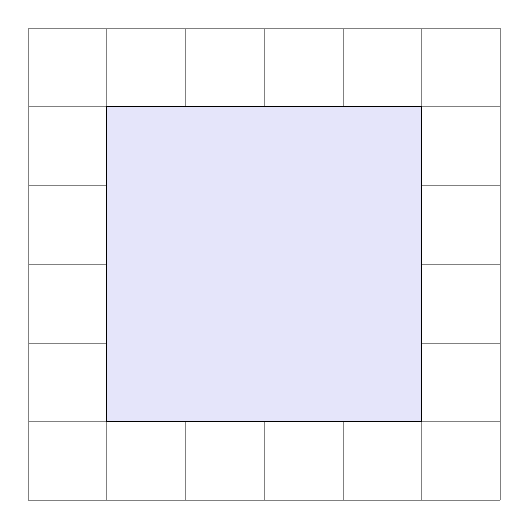
\begin{tikzpicture}
  \draw[step=1cm,gray,very thin] (0,0) grid (6,6);
  \draw[fill=lavender] (1,1) rectangle (5,5);
\end{tikzpicture}
\end{center}

\ \\
\definecolor{mondrian_red}{RGB}{226,25,10}
\definecolor{mondrian_blue}{RGB}{27,81,227}
\definecolor{mondrian_yellow}{RGB}{238,208,17}

\begin{center}
\begin{tikzpicture}
	\draw[fill=white,line width=1mm] (2,6) rectangle(3,8);
	\draw[fill=white,line width=1mm] (2,3) rectangle(3,6);
  \draw[fill=mondrian_yellow,line width=1mm] (2,1) rectangle(3,3);
  \draw[fill=white,line width=1mm] (3,1) rectangle(5,2);
  \draw[fill=black,line width=1mm] (3,2) rectangle(5,4);
  \draw[fill=white,line width=1mm] (5,2) rectangle(7,3);
  \draw[fill=white,line width=1mm] (5,1) rectangle(9.6,1.6);
  \draw[fill=mondrian_blue,line width=1mm] (7,1.6) rectangle(9.6,3);
  \draw[fill=black,line width=1mm] (5,1.6) rectangle(7,2);
  \draw[fill=white,line width=1mm] (7,3) rectangle(9.6,4);
  \draw[fill=white,line width=1mm] (5,3) rectangle(7,4);
  \draw[fill=mondrian_red,line width=1mm] (3,4) rectangle(7,8);
  \draw[fill=white,line width=1mm] (7,4) rectangle(8.3,6);
  \draw[fill=white,line width=1mm] (8.3,4) rectangle(9.6,6);
  \draw[fill=mondrian_yellow,line width=1mm] (7,6) rectangle(9.6,8);
\end{tikzpicture}
\end{center}

\pagebreak

\begin{c++}
    #include<iostream>
    using namespace std;

    int main(){
      /* insert comment here */
      int n;
      while (cin >> n){
        cout << n << endl;
      }
    }
\end{c++}
\ \\
\begin{cbox}
  \label{mondrian}
  \begin{center}
  \begin{tikzpicture}
  	\draw[fill=white,line width=1mm] (2,6) rectangle(3,8);
  	\draw[fill=white,line width=1mm] (2,3) rectangle(3,6);
    \draw[fill=mondrian_yellow,line width=1mm] (2,1) rectangle(3,3);
    \draw[fill=white,line width=1mm] (3,1) rectangle(5,2);
    \draw[fill=black,line width=1mm] (3,2) rectangle(5,4);
    \draw[fill=white,line width=1mm] (5,2) rectangle(7,3);
    \draw[fill=white,line width=1mm] (5,1) rectangle(9.6,1.6);
    \draw[fill=mondrian_blue,line width=1mm] (7,1.6) rectangle(9.6,3);
    \draw[fill=black,line width=1mm] (5,1.6) rectangle(7,2);
    \draw[fill=white,line width=1mm] (7,3) rectangle(9.6,4);
    \draw[fill=white,line width=1mm] (5,3) rectangle(7,4);
    \draw[fill=mondrian_red,line width=1mm] (3,4) rectangle(7,8);
    \draw[fill=white,line width=1mm] (7,4) rectangle(8.3,6);
    \draw[fill=white,line width=1mm] (8.3,4) rectangle(9.6,6);
    \draw[fill=mondrian_yellow,line width=1mm] (7,6) rectangle(9.6,8);
  \end{tikzpicture}
  \end{center}
\end{cbox}

\begin{cbox}
  \label{code}
  Integer vitae tincidunt nisi. Nam enim eros, suscipit eu luctus quis, vulputate fermentum ante.
  Nullam pulvinar velit ac nunc mollis semper. Ut tristique vitae sapien non commodo. Nullam blandit, ex quis elementum gravida, est
  turpis vehicula mi, ut ultricies ligula felis in ipsum.
  \begin{c++}
    int main(){
      /* insert comment here */
      int n;
      while (cin >> n){
        cout << n << endl;
      }
    }
  \end{c++}
\end{cbox}

You can of course refer to the above boxes using \ref{mondrian} and \ref{code}, but
it only references mycounter (you need to combine counters if you want the chapter number
to appear as well).

\end{document}
